\chapter{Fusion}
\label{chap:fusion}

This chapter will outline the principles behind
\textit{producer-consumer} loop fusion, describe their implementation
in the \LO{} compiler, and discuss possible complications and
restrictions of my handling of loop fusion.

In producer-consumer fusion, the aim is to merge (or \textit{fuse})
two loops, where the output of the first loop -- the producer -- is
used as input to the second -- the consumer.  We currently only fuse
loops that are expressed via SOACs, not the \texttt{loop}-notation.
The reason for this is to simplify analysis, as it can be hard to
determine in which cases arbitrary \texttt{do}-loops can be combined,
whereas it is possible to define simple rules for how and when SOACs
can be fused.

As a simple case, we can fuse the two loops in
\[
\texttt{(map~$f$)~$\circ$~(map~$g$)}
\]
and get
\[
\texttt{map~$(f~\circ~g)$},
\]
thus removing the need to construct an intermediary array for the
result of \texttt{map~$g$}, and in the context of GPGPU, reducing the
likelyhood of global memory accesses, which exhibit high memory
latency.  We will write ``$c_{1}$-$c_{2}$ fusion'' for the case where
a fusion is formed with $c_{1}$ as the producer and $c_{2}$ as the
consumer.  Therefore, the previous example would be
``\texttt{map}-\texttt{map}''-fusion.

The rules by which we combine SOACs through fusion is called our
\textit{fusion algebra}.  We aim at preserving the parallelism of the
resulting expressions.

\Cref{sec:fusionalgebra} describes superficially which
producer-consumer pairs can be fused, as well as the form of the
resulting SOAC.  \Cref{sec:invalidfusion} goes into greater detail on
invalid fusion, and \cref{sec:whentofuse} covers cases in which fusion
may actually be detrimental to performance.

\section{Fusion in \LO{}}
\label{sec:fusion-in-l0}

The language used to describe the fusion algorithm in this chapter is
\texttt{let}-normalised, internal \LO{}, as described in
\cref{chap:internal,sec:let-normalisation}.  We will also assume that
all instances of \texttt{replicate(n,x)} have been rewritten as
\texttt{map(fn~t~(int~i)~=>~x,~iota(n))}\footnote{In the actual
  implementation, we convert these back into \texttt{replicate}
  expressions if they are not fused, but for clarity the bookkeeping
  necessary is elided in this presentation.}.  For clarity, expository
examples will use the external \LO{}.

\begin{figure}
  \begin{center}
    \begin{tabular}{c|c}
      \textbf{Producers} & \textbf{Consumers} \\\hline
      \texttt{map} & \texttt{map} \\\hline
      & \texttt{reduce} \\\hline
      & \texttt{scan} \\\hline
      \texttt{filter} & \texttt{filter} \\\hline
      & \texttt{redomap} \\\hline
    \end{tabular}
  \end{center}
  \caption{Producers and consumers in \LO}
  \label{fig:producers-consumers}
\end{figure}

\Cref{fig:producers-consumers} lists which \LO{} SOACs are producers,
which are consumers, and which are both.  In particular, note that
even if we have a \texttt{reduce}-expression returning an array, this
does not mean that the \texttt{reduce}-expression is a producer -
because, in our algebra, it cannot be fused into another SOAC
expression.  The reason is that the output of the reduction is only
fully known after the final input array element has been processed.
Consider the following program:

\begin{colorcode}
let b = reduce(fn [int] ([int] acc, int x) =>
                 map(op + (x), acc),
               iota(10), a) in
map(f, b)
\end{colorcode}

The contents of the array \texttt{b} is not determined until the very
last element of \texttt{a} has been processed, and thus fusion with
the \texttt{map}-expression cannot take place.  While it is possible
to use \texttt{reduce} in a way that could theoretically be fused with
a consumer (for example by using it to simulate \texttt{map}), the
analysis necessary to determine whether a given reduction is fusible
would be quite onerous, and likely not useful in any but contrived
examples, such as the above-mentioned simulation of \texttt{map}.

In this way, \texttt{reduce} differs from \texttt{map}, in which each
element of the output is calculated from one element of the input ---
a classic case of data-parallelism.

Even if we have a producer-consumer-pair, not all such pairs
\textit{can} be fused, and not all are \textit{desirable} to fuse.
For instance, \texttt{filter}-\texttt{map} fusion is not possible,
although \texttt{filter}-\texttt{reduce} is.  The reason is that, with
the former, the size of the \texttt{map}-output is the same as the
size of its input, yet the size of the output of \texttt{filter}
cannot be known in advance, which precludes an efficient fused form.

\subsection{Fusion algebra}
\label{sec:fusionalgebra}

In this section, we will give an informal introduction to which SOACs
can be fused, as well as the form of the result.  In order to preserve
clarity, we will not go into great detail until
\cref{sec:fusion-rules}.

\subsubsection{\texttt{map-map} fusion}

The quintessential example of fusion is composing two consecutive
\texttt{map} operations into a single \texttt{map}, as follows:

\begin{colorcode}
let \{x1, x2\} = mapT(f, a1)
in  mapT(g, x1, y)
    \emphh{\mymath{\Downarrow}}
mapT(fn \mymath{\beta} (\mymath{\alpha\myindx{1}} a1\mymath{\myindx{i}}, \mymath{\alpha\myindx{2}} y\mymath{\myindx{i}}) =>
      let \{x1\mymath{\myindx{i}}, x2\mymath{\myindx{i}}\} = f(a1\mymath{\myindx{i}})
      in  g(x1\mymath{\myindx{i}}, y\mymath{\myindx{i}})
    , a1, y )
\end{colorcode}

\subsubsection{\texttt{replicate} fusion}

\texttt{replicate} is an interesting case.  We wish to always be able
to fuse replicate into a consumer, like this:

\begin{colorcode}
let x = replicate(N,a) in
mapT(f, x) in
    \emphh{\mymath{\Downarrow}}
mapT(fn \mymath{\beta\myindx{1}} (int i) =>
       f(a), b)
\end{colorcode}

And indeed, this can be done through ordinary \texttt{map}-fusion if
\texttt{replicate(N,a)} is first rewritten to \texttt{map} as
described in \cref{sec:fusion-in-l0}.

\subsubsection{\texttt{map-reduce} and \texttt{map-scan} fusion}

The result of \texttt{map}-\texttt{reduce}-fusion is normally
\texttt{redomap}.

\begin{colorcode}
let \{x1, x2\} = mapT(f, a1)
in  reduceT(\mymath{\oplus},e\mymath{\myindx{1}},e\mymath{\myindx{2}}, x1,y)
    \emphh{\mymath{\Downarrow}}
redomapT(\mymath{\oplus}
, fn (\mymath{\beta\myindx{1}},\mymath{\beta\myindx{2}}) ( \mymath{\beta\myindx{1}} e\mymath{\myindx{1}}, \mymath{\beta\myindx{2}} e\mymath{\myindx{2}}
             , \mymath{\alpha\myindx{1}} a1\mymath{\myindx{i}},\mymath{\alpha\myindx{2}} y\mymath{\myindx{i}})
   => let \{x1\mymath{\myindx{i}}, x2\mymath{\myindx{i}}\} = f(a1\mymath{\myindx{i}})
      in  \mymath{\oplus}(e\mymath{\myindx{1}},e\mymath{\myindx{2}},x1\mymath{\myindx{i}},y\mymath{\myindx{i}})
, (e\mymath{\myindx{1}}, e\mymath{\myindx{2}}), a1, y )
\end{colorcode}

In general, we cannot fuse \texttt{map} and \texttt{reduce} to another
\texttt{reduce}, as the accumulator type of a reduction must match the
element type of the input array. Adding the input of the \texttt{map}
to the input of the \texttt{reduce} may violate this requirement, as
demonstrated on \cref{fig:map-reduce-error}.

\begin{figure}
\begin{center}
\begin{colorcode}
let \{c\} = mapT(fn \{int\} (int x, int y) => \{x+y\},
                 a, b) in
reduceT(op +, \{0\}, c)
  \(\emphh{\Downarrow}\)
reduceT(fn int (int acc, int x, int y) => acc + x + y,
        \{0\}, a, b) \emp{// Type error, as accumulator}
                   \emp{// type must match array input type}
\end{colorcode}
\end{center}

\caption{Cannot fuse to \texttt{reduce} (but \texttt{redomap} would be valid)}
\label{fig:map-reduce-error}
\end{figure}

The solution is to first rewrite \texttt{reduceT($\oplus$,$x$,$a$)} to
\texttt{redomapT($\oplus$,$\oplus$,$x$,$a$)}, since we can always fuse
\texttt{map} with \texttt{redomap}:

\begin{colorcode}
let \{x1, x2\} = mapT(f, a1)
in  redomapT(\mymath{\oplus}, g, e, x1, y)
    \emphh{\mymath{\Downarrow}}
redomapT(\mymath{\oplus}
, fn \mymath{\beta} (\mymath{\beta} e, \mymath{\alpha\myindx{1}} a1\mymath{\myindx{i}}, \mymath{\alpha\myindx{2}} y\mymath{\myindx{i}})
   => let \{x1\mymath{\myindx{i}}, x2\mymath{\myindx{i}}\} = f(a1\mymath{\myindx{i}})
      in  g(e, x1\mymath{\myindx{i}}, y\mymath{\myindx{i}})
, e, a1, y )
\end{colorcode}

However, there are a few rare cases where we can fuse \texttt{map} and
\texttt{reduce} to \texttt{reduce}.  This only happens when the
\textit{input} to the map has the same count and types as the outputs
of the \texttt{map} that are being used as input to the
\texttt{reduce}.

\begin{colorcode}
let \{x\cindx{1}, x\cindx{2}\} = mapT(f, a\cindx{1}, a\cindx{2})
in  reduceT(\mymath{\oplus},\{e\cindx{1}, e\cindx{2}, e\cindx{3}\}, x\cindx{1}, x\cindx{2}, y)
    \emphh{\mymath{\Downarrow}}
reduceT(fn (\(\alpha\myindx{1}\),\(\alpha\myindx{2}\)) ( \(\alpha\myindx{1}\) x\cindx{1}, \(\alpha\myindx{2}\) x\cindx{2}, \(\alpha\myindx{3}\) x\cindx{3},
            \(\alpha\myindx{1}\) ai\cindx{1}, \(\alpha\myindx{2}\) ai\cindx{2}, \(\alpha\myindx{3}\) ye) =>
          let \{x\cindx{1}, x\cindx{2}\} = f(ae\cindx{1}, ae\cindx{2})
          in  \mymath{\oplus}(x\cindx{1}, x\cindx{2}, x\cindx{3}, x\cindx{1}, x\cindx{2}, ye)
        , \{e\cindx{1}, e\cindx{2}, e\cindx{3}\}, a\cindx{1}, a\cindx{2}, y)
\end{colorcode}

In fact, under these circumstances we can also fuse \texttt{map} with
\texttt{scan}:

\begin{colorcode}
let \{x\cindx{1}, x\cindx{2}\} = mapT(f, a\cindx{1}, a\cindx{2})
in  scanT(\mymath{\oplus},\{e\cindx{1}, e\cindx{2}, e\cindx{3}\}, x\cindx{1}, x\cindx{2}, y)
    \emphh{\mymath{\Downarrow}}
scanT(fn (\(\alpha\myindx{1}\),\(\alpha\myindx{2}\)) ( \(\alpha\myindx{1}\) x\cindx{1}, \(\alpha\myindx{2}\) x\cindx{2}, \(\alpha\myindx{3}\) x\cindx{3},
          \(\alpha\myindx{1}\) ai\cindx{1}, \(\alpha\myindx{2}\) ai\cindx{2}, \(\alpha\myindx{3}\) ye) =>
        let \{x\cindx{1}, x\cindx{2}\} = f(ae\cindx{1}, ae\cindx{2})
        in  \mymath{\oplus}(x\cindx{1}, x\cindx{2}, x\cindx{3}, x\cindx{1}, x\cindx{2}, ye),
      \{e\cindx{1}, e\cindx{2}, e\cindx{3}\}, a\cindx{1}, a\cindx{2}, y)
\end{colorcode}

It should be clear that the composed function is still associative, as
required by \texttt{scan} and \texttt{reduce}.

\subsubsection{\texttt{filter-filter} fusion}

Fusing \texttt{filter-filter} is quite simple - it's a new
\texttt{filter} SOAC where both of the filter functions must return
true for each element.  However, we can only perform the fusion if the
input set of the consumer is a subset of the output set of the
producer.  Put another way, the consumer must accept input from no
other source than the producer involved in the fusion.\footnote{The
  implementation in the \LO{} compiler is currently even more
  restrictive, in that the input set of the consumer must match the
  output set of the producer \textit{exactly}.  Fixing this oversight
  is left as an exercise for the author.}

\begin{colorcode}
let \{x\cindx{1},x\cindx{2}\}=filterT(c\cindx{1},a\cindx{1},a\cindx{2}) in
let \{y\} = filterT(c\cindx{2}, x\cindx{1}) in
...
    \emphh{\mymath{\Downarrow}}
let \{y, _\} = filterT(fn bool (\(\alpha\myindx{1}\) ai\cindx{1},\(\alpha\myindx{2}\) ai\cindx{2}) =>
                       if   c\cindx{1}(ai\cindx{1}, ai\cindx{2})
                       then c\cindx{2}(ai\cindx{1})
                       else False,
                     a\cindx{1}, a\cindx{2} ) in
...
\end{colorcode}

As a bit of a technical curiosity, we are forced to use an
\texttt{if}-expression, as the \texttt{\&\&} operator in \LO{} is not
short-circuiting.

\subsubsection{\texttt{filter-reduce} fusion}

We can fuse \texttt{filter} with \texttt{reduce} and obtain
\texttt{reduce} \textit{only} in the case where the input set of the
\texttt{reduce} is equal to the output set of the \texttt{filter}.

\begin{colorcode}
let \{x\} = filterT(c, a) in
reduceT(\mymath{\oplus}, e, x)
    \emphh{\mymath{\Downarrow}}
reduceT(fn \(\beta\) (\(\beta\) e, \(\beta\) ai) =>
          if c(ai) then \(\oplus\)(e,ai) else e,
        \{e\}, a)
\end{colorcode}

We can fuse \texttt{filter} with \texttt{reduce} and obtain
\texttt{redomapT} if the input set of the \texttt{reduce} is included
in the output set of the \texttt{filter}.

\begin{colorcode}
let \{x1,x2\} = filterT(c, a\cindx{1}, a\cindx{2})
in  reduceT(\(\oplus\), \{e\}, x\cindx{1})
    \emphh{\mymath{\Downarrow}}
redomapT(\(\oplus\),
         fn \(\beta\) (\(\beta\) e, \(\alpha\myindx{1}\) ai\cindx{1}, \(\alpha\myindx{2}\) ai\cindx{2}) =>
           if c(ai\cindx{1}, ai\cindx{2})
           then \(\oplus\)(e, ai\cindx{1})
           else e,
         \{e\}, a\cindx{1}, a\cindx{2})
\end{colorcode}

\subsubsection{\texttt{filter-redomap} fusion}

Similarly, we can fuse \texttt{filter} with \texttt{redomapT} and
obtain \texttt{redomapT} if the input set of the \texttt{reduce} is
included in the output set of the \texttt{filter}.

\begin{colorcode}
let \{x\cindx{1},x\cindx{2}\}=filterT(c, a\cindx{1}, a\cindx{2})
in  redomapT(\(\oplus\), g, \{e\}, x\cindx{1})
    \emphh{\(\Downarrow\)}
redomapT(\(\oplus\),
         fn \(\beta\) (\(\beta\) e, \(\alpha\myindx{1}\) ai\cindx{1}, \(\alpha\myindx{2}\) ai\cindx{2}) =>
           if c(ai\cindx{1}, ai\cindx{2})
           then g(e, ai\cindx{1})
           else e,
         \{e\}, a\cindx{1}, a\cindx{2} )
\end{colorcode}

\subsection{Invalid fusion}
\label{sec:invalidfusion}

We must be careful not to violate the uniqueness rules when performing
fusion.  For example, consider the following program.

\begin{colorcode}
let b = map(f, a) in
let c = a with [i] <- x in
map(g, b)
\end{colorcode}

Without the constraints imposed upon us by the semantics of in-place
modification, we could fuse to the following program.

\begin{colorcode}
let c = a with [i] <- x in
map(g \(\circ\) f, a)
\end{colorcode}

However, this results in a violation of Uniqueness Rule 1, and the
resulting program is thus invalid.  In general, we must track the
possible execution paths from the producer-SOAC to the consumer-SOAC,
and only fuse if none of the inputs of the producer have been consumed
(in the uniqueness type sense of the word) by a \texttt{let-with} or
function call on any possible execution paths.  This is easier than it
may appear at first glance, as the fusion algorithm will only fuse
when the consumer is within the lexical scope of the producer anyway.

\subsection{When to fuse}
\label{sec:whentofuse}

Even when fusion is possible, it may not be beneficial, and may be
harmful to overall performance in the following cases.

\begin{description}[style=nextline]
\item[Computation may be duplicated.]

In the program
\begin{colorcode}
let x = map(f, a) in
\{map(g, x), map(h, x)\}
\end{colorcode}
fusing the \texttt{x}-producer into the two consumers will double the
number of calls to the function \texttt{f}, which might be expensive.
The implementation in the \LO{} compiler will currently only fuse if
absolutely no computation is duplicated, although this is likely too
conservative.  Duplicating cheap work, for example functions that use
only primitive operations on scalars, is probably not harmful to
overall performance, although we have not investigated this
fully.\fxnote{Reference someone who has.}

In general, in the context of GPU, the tradeoff between duplicating
computation and increasing communication is not an easy problem to
solve.  Accessing global memory can be more than a hundred times
slower than accessing local (register) memory, hence duplicating
computation is in many cases preferable.

\item[Can reduce memory locality.]

  Consider a simple case of fusing
  \texttt{(map~$f$)~$\circ$~(map~$g$)}.  When $g$ is executed for an
  element of the input array, neighboring elements will be put into
  the cache, making them faster to access.  This exhibits good data
  locality.  In contrast, the composed function $f~\circ~g$ will
  perform more work after accessing a given input element, increasing
  the risk that the input array may be evicted from the cache before
  the next element is to be used.  On GPUs, there is the added risk of
  the kernel function exercising additional register pressure, which
  may reduce hardware occupancy (thus reducing latency hiding) by
  having fewer computational cores active.  In this case, it may be
  better to execute each of the two \texttt{map}s as separate kernels.

  The \LO{} compiler does not currently handle this problem, as it is
  envisioned that a later (and as-of-yet unimplemented) transformation
  will perform \textit{loop distribution} (sometimes called
  \textit{loop fission}).  This step is necessary in any case, as it
  can be used to improve the degree of parallelism, compared to the
  original program.  \Cref{fig:loop-distribution} demonstrates a fully
  fused \texttt{map} where the degree of parallelism can be improved
  by distributing the inner reductions out of the loop.  In the
  original program, the inner map had to wait for the two reductions
  to finish computing \texttt{x} and \texttt{y} before executing its
  inner loop, whereas the distributed program consists of three
  parallel loop nests.
\end{description}

The fusion algorithm is currently designed to fuse as much as
possible, although without duplicating computation.

\begin{figure}
\begin{center}
\begin{bcolorcode}
map(fn int ([int] r) =>
      let x = reduce(f, 0, r) in
      let y = reduce(g, 0, r) in
      map(h(x,y), r),
    a)
\end{bcolorcode}

$\Downarrow$

\begin{bcolorcode}
let xs = map(reduce(f,0),a) in
let ys = map(reduce(g,0),a) in
map(fn [int] (\{int,int,[int]\} t) =>
      let \{r,x,y\} = t in
      map(h(x,y), r),
    zip(a,xs,ys))
\end{bcolorcode}
\end{center}
\caption{Loop distribution}
\label{fig:loop-distribution}
\end{figure}

\section{Composition}

\newcommand\mapcompose[7]{ (#1,#2) \underset{\texttt{map}}{\overset{#3}\circ}(#4,#5) \Rightarrow (#6,#7) }
\newcommand\filtercompose[7]{ (#1,#2) \underset{\texttt{filter}}{\overset{#3}\circ}(#4,#5) \Rightarrow (#6,#7) }
\newcommand\foldcompose[7]{ (#1,#2) \underset{\texttt{fold}}{\overset{#3}\circ}(#4,#5) \Rightarrow (#6,#7) }
\newcommand\inputmapping[0]{\mathcal{I}}
\newcommand\arrparams[1]{\textrm{params}(#1)}

To begin the exposition of the precise mechanics of fusion, we will
present the mechanics behind composing the functions involved in a
fusion operation.  For example, consider the trivial example of
\texttt{map}-\texttt{map}-fusion.  In principle, the equation seems
simple enough:
\[
\texttt{map}\ f \circ \texttt{map}\ g = \texttt{map}\ (f \circ g).
\]
However, while the intuition behind the above equation is correct, it
is woefully imprecise.  Fusion in \LO{} is not performed on simple
\texttt{map}s that take input from only one other \texttt{map}, but
complex \texttt{mapT}s that may take input from several sources, where
only some may be fusible.  Hence, a more detailed elaboration is
necessary.

This section will describe various ways of combining the functions
used in SOACs, as appropriate for different cases of fusion.  In
\cref{sec:fusion-rules}, we will describe the rules used for fusion of
full SOAC expressions.

In this section, we will assume that each output of a producer is used
exactly once in every relevant \texttt{redomap}- and
\texttt{map}-consumer.  This assumption can be provided through
trivial rewriting prior to performing function composition, as
illustrated on \cref{fig:single-input-transform}.  We gain the
property that each output of the producer is bound to exactly one
parameter of the consumer's function, making it easier to describe the
relationship between producer and consumer.\footnote{In the actual
  implementation, this transformation is not done.  Instead, the
  composition uses more complicated bookkeeping, but presenting all
  details would obscure the exposition of the central mechanism.}

\begin{figure}
\begin{center}
\begin{bcolorcode}
let \{x, y, z\} = mapT(f, a) in
mapT(fn int (int a, int b, int c) => \(e\), x, y, x)
\end{bcolorcode}

$\Downarrow$

\begin{bcolorcode}
let \{x, y, z\} = mapT(f, a) in
mapT(fn int (int a, int b, int d) =>
       let c = a in \(e\),
     x, y, z)
\end{bcolorcode}
\end{center}
\caption{Single-input transformation}
\label{fig:single-input-transform}
\end{figure}

The presentation will be of the form of \textit{judgements}.  To skip
ahead a bit, we will write the \texttt{map}-composition of two
functions as
\[
\boxed{
\mapcompose{l_{b}}{e_{b_{1}},\ldots,e_{b_{m}}}{o_1,\ldots,o_k}{l_{a}}{e_{a_{1}},\ldots,e_{a_{n}}}{l_{r}}{e_{r_{1}},\ldots,e_{r_{l}}}
}.
\]
This judgement is said to \textit{hold} if the preconditions specified
for the judgement are upheld.  The preconditions for a given
judgement, if any, will be listed when the judgement is defined below.

\subsection{\texttt{map}-\texttt{map} composition}
\label{sec:map-map-composition}

We are given two functions:
\[
l_{a}\equiv\texttt{fn $t_{a_{r}}$ ($p_{a_{1}}$, \ldots, $p_{a_{n}}$) => $e_{a}$}
\]
whose inputs are \texttt{$e_{a_{1}}$,\ldots,$e_{a_{m}}$} and whose
outputs are \texttt{$o_1$,\ldots,$o_k$}; and
\[
l_{b}\equiv\texttt{fn $t_{b_{r}}$ ($p_{b_{1}}$, \ldots, $p_{b_{m}}$) => $e_{b}$},
\]
whose inputs are \texttt{$e_{b_{1}}$,\ldots,$e_{b_{m}}$}.

The goal is to compute a function
\[
l_{r} \equiv \texttt{fn $t_{b_{r}}$ ($p_{r_{1}}$, \ldots, $p_{r_{l}}$)
=> $e_{r}$}
\]
that corresponds to the intuitive notion of the composition $l_{b}
\circ l_{a}$.

For notational convenience, we define the following sets of parameters
of the two functions.
\[
\arrparams{l_{a}} = \{p_{a_{1}}, \ldots, p_{a_{n}}\}
\]
\[
\arrparams{l_{b}} = \{p_{b_{1}}, \ldots, p_{b_{m}}\}
\]

If the inputs of $l_{b}$ are disjoint from the outputs of $l_{a}$,
then we are done, and $l_{r} = l_{b}$.  Otherwise, there is a
non-empty mapping
\[
\inputmapping(o_{i}) = p_{b_{j}} \quad \textrm{when $o_{i} = e_{b_{j}}$}
\]
of outputs of $l_{a}$ to the corresponding parameters of $l_{b}$.  The
parameters (and corresponding inputs) to the desired function $l_{r}$
are the parameters of $l_{b}$, except those in $\inputmapping$,
concatenated with the parameters of $l_{a}$:
\[
\{e_{r_{1}},\ldots,e_{r_{l}}\} = \arrparams{l_{r}} = (\arrparams{l_{b}} \backslash \delta) \oplus \arrparams{l_{a}}
\]
where $\delta$ are the parameters $p_{b_{j}}$ in the range of
$\inputmapping$.

The body of $l_{r}$ is then defined as follows:
\[
e_{r} \equiv \texttt{let \{$\inputmapping(o_{1})$,\ldots,$\inputmapping(o_{k})$\} = $e_{a}$ in $e_{b}$}
\]

We will refer to this entire operation as:
\[
\mapcompose{l_{b}}{e_{b_{1}},\ldots,e_{b_{m}}}{o_1,\ldots,o_k}{l_{a}}{e_{a_{1}},\ldots,e_{a_{n}}}{l_{r}}{e_{r_{1}},\ldots,e_{r_{l}}}
\]

\subsection{\texttt{filter}-\texttt{filter} composition}

We do not have \texttt{fold} per se in \LO{}, but this method of
composition is used for both \texttt{reduce} and the
\texttt{fold}-like semantics of \texttt{redomap}, hence the name.

We are given two functions:
\[
l_{a}\equiv\texttt{fn \{bool\} ($p_{a_{1}}$, \ldots, $p_{a_{n}}$) => $e_{a}$}
\]
which take as inputs \texttt{$e_{a_{1}}$,\ldots,$i_{e_{n}}$}, and whose
outputs are \texttt{$o_1$,\ldots,$o_k$}; and
\[
l_{b}\equiv\texttt{fn \{bool\} ($p_{b_{1}}$, \ldots, $p_{b_{n}}$) => $e_{b}$},
\]
whose inputs are \texttt{$e_{b_{1}}$,\ldots,$e_{b_{n}}$}.

\textbf{Precondition:} Every input $e_{b_{i}}$ must correspond to some
output $o_{j}$, and every output $o_{i}$ must correspond to some input
$e_{b_{i}}$.  That is, the producer set of $l_{a}$ is equal to the
input set of $l_{b}$.  Or to put it another way, $l_{b}$ takes input
from no other source.

The goal is to compute a function
\[
l_{r} \equiv \texttt{fn \{bool\} ($p_{a_{1}}$, \ldots, $p_{a_{n}}$)
=> $e_{r}$}
\]
whose inputs are \texttt{$i_{r_{1}}$,\ldots,$i_{r_{l}}$}, that
corresponds to the intuitive composition of $l_{a} \wedge l_{b}$.
Note that the parameters are the same as for $l_{a}$, which means that
we have to explicitly create a \texttt{let}-binding for the names of
the parameters of $l_{b}$ or they will be free in $e_{b}$.  To this end,
define the mapping
\[
\inputmapping(o_{i}) = p_{b_{j}} \quad \textrm{when $o_{i} = e_{b_{j}}$}.
\]

The body of $l_{r}$ is now definable as
\begin{align*}
e_{r} \equiv\quad&\texttt{let \{$ok$\} = $e_{a}$ in $ok$ \&\&} \\
& \texttt{let \{$\inputmapping(o_{1})$,\ldots,$\inputmapping(o_{k})$\} = \{$p_{a_{i}}$,\ldots,$p_{a_{n}}$\} in $e_{b}$}
\end{align*}
where $ok$ is some fresh variable.

We will refer to this entire operation as:
\[
\filtercompose{l_{b}}{e_{b_{1}},\ldots,e_{b_{n}}}{o_{1},\ldots,o_{k}}{l_{a}}{e_{a_{1}},\ldots,e_{a_{n}}}{l_{r}}{e_{a_{1}},\ldots,e_{a_{n}}}
\]

\subsection{\texttt{filter}-\texttt{fold} composition}

We are given two functions:
\[
l_{a}\equiv\texttt{fn \{bool\} ($p_{a_{1}}$, \ldots, $p_{a_{n}}$) => $e_{a}$}
\]
which take as inputs \texttt{$e_{a_{1}}$,\ldots,$i_{e_{n}}$}, and whose
outputs are \texttt{$o_1$,\ldots,$o_k$}; and
\[
l_{b}\equiv\texttt{fn $t_{b_{r}}$ ($u_{b_{1}}$, \ldots, $u_{b_{m}}$, $p_{b_{1}}$, \ldots, $p_{b_{n}}$) => $e_{b}$},
\]
whose inputs are \texttt{$e_{b_{1}}$,\ldots,$e_{b_{n}}$}.

\textbf{Precondition:} Every input $e_{b_{i}}$ corresponds to some
output $o_{j}$, and every output $o_{i}$ corresponds to some input
$e_{b_{i}}$.  That is, the producer set of $l_{a}$ is equal to the
input set of $l_{b}$.  Or to put it another way, $l_{b}$ takes input
from no other source.  The $u_{b}$s are accumulator parameters that do
not correspond to an array input.

The goal is to compute a function
\[
l_{r} \equiv \texttt{fn $t_{b_{r}}$ ($p_{r_{1}}$, \ldots, $p_{r_{l}}$)
=> $e_{r}$}.
\]

Note that the parameters are the same as for $l_{a}$, which means that
we have to explicitly create a \texttt{let}-binding for the names of
the parameters of $l_{b}$ before $e_{b}$ makes sense.  To this end,
define the mapping
\[
\inputmapping(o_{i}) = p_{b_{j}} \quad \textrm{when $o_{i} = e_{b_{j}}$}.
\]

The body of $l_{r}$ is now definable as
\begin{align*}
e_{r} \equiv\quad&\texttt{let \{$ok$\} = $e_{a}$ in if $ok$} \\
& \texttt{then let \{$\inputmapping(o_{1})$,\ldots,$\inputmapping(o_{k})$\} = \{$p_{a_{i}}$,\ldots,$p_{a_{n}}$\} in $e_{b}$} \\
& \texttt{else \{$u_{b_{1}}$, \ldots, $u_{b_{m}}$\}}
\end{align*}
where $ok$ is some fresh variable.

We will refer to this entire operation as:
\[
\foldcompose{l_{b}}{e_{b_{1}},\ldots,e_{b_{n}}}{o_{1},\ldots,o_{k}}{l_{a}}{e_{a_{1}},\ldots,e_{a_{n}}}{l_{r}}{e_{a_{1}},\ldots,e_{a_{n}}}
\]

\section{Fusion rules}
\label{sec:fusion-rules}

\newcommand\fusesto[4]{\bfrac{#2\overset{#1}{\leadsto}#3}{\Rightarrow #4}}

With function composition defined, we can define fusion rules for
SOACs.  We present fusion as a judgement
\[
\boxed{
\fusesto{os}{producer}{consumer}{result}
}.
\]
This means that $producer$, which produces outputs $os$, can be fused
with $consumer$, yielding $result$ as the combined SOAC.  Valid
judgements of this form are given by the following inference rules,
which should mostly be intuitive.

\begin{align*}
  \nfrac{
    \mapcompose{l_{b}}{\overline{es_{b}}}{\overline{os}}{l_{a}}{\overline{es_{a}}}{l_{r}}{\overline{es_{r}}}
  }{
    \fusesto
    {os}
    {\texttt{mapT($l_{a}$,$\overline{es_a}$)}}
    {\texttt{mapT($l_{b}$,$\overline{es_b}$)}}
    {\texttt{mapT($l_{r}$,$\overline{es_r}$)}}
  }
  \tagsc{Fuse-Map-Map}
\end{align*}

\begin{align*}
  \nfrac{
    \mapcompose
    {l_{b}}
    {\overline{es_{b}}}
    {\overline{os}}
    {l_{a}}
    {\overline{es_{a}}}
    {l_{r}}
    {\overline{es_{r}}}
  }{
    \fusesto
    {os}
    {\texttt{mapT($l_{a}$,$\overline{es_a}$)}}
    {\texttt{scanT($l_{b}$,\{$\overline{us}$\},$\overline{es_b}$)}}
    {\texttt{scanT($l_{r}$,\{$\overline{us}$\},$\overline{es_r}$)}}
  } \quad \mbox{($\overline{es_{a}}$ = $\overline{es_{b}}$)}
  \tagsc{Fuse-Map-Scan}
\end{align*}

Fusing \texttt{map}-\texttt{reduce} and
\texttt{filter}-\texttt{reduce} is usually done by first rewriting
\texttt{reduce} to \texttt{redomap}, although when the producer-output
and consumer-input match exactly, \texttt{filter}-\texttt{reduce} can
fuse to \texttt{reduce}.

\begin{align*}
  \nfrac{
    \fusesto
    {\overline{os}}
    {\texttt{filterT($l_{a}$,$\overline{es_a}$)}}
    {\texttt{redomapT($l_{b}$,$l_{b}$,\{$\overline{us}$\},$\overline{es_b}$)}}
    {\texttt{redomapT($l_{b}$,$l_{r}$,\{$\overline{us}$\},$\overline{es_r}$)}}
  }{
    \fusesto
    {os}
    {\texttt{filterT($l_{a}$,$\overline{es_a}$)}}
    {\texttt{reduceT($l_{b}$,\{$\overline{us}$\},$\overline{es_b}$)}}
    {\texttt{reduceT($l_{r}$,\{$\overline{us}$\},$\overline{es_a}$)}}
  } \quad (\overline{es_{b}} \subseteq \overline{os})
  \tagsc{Fuse-Filter-Reduce-1}
\end{align*}

Note that \textsc{Fuse-Filter-Reduce-1} has a side condition that
implies that the types of $\overline{es_{a}}$ are equal to the types of $\overline{es_{b}}$.
This permits us to keep the result as a \texttt{reduceT} rather than a
\texttt{redomapT}.

\begin{align*}
  \nfrac{
    \mapcompose
    {\texttt{fn $t_{b_{r}}$ ($\overline{ps_{b}}$) => $e_{b}$}}
    {\overline{es_{b}}}
    {\overline{os}}
    {l_{a}}
    {\overline{es_{a}}}
    {\texttt{fn $t_{b_{r}}$ ($\overline{ps_{r}}$) => $e_{r}$}}
    {\overline{es_{r}}}
  }{
    \fusesto
    {os}
    {\texttt{mapT($l_{a}$,$\overline{es_{a}}$)}}
    {\texttt{redomapT($\oplus$,\texttt{fn $t_b$ ($\overline{us_{b}}$, $\overline{ps_{b}}$) => $e_{b}$},\{$\overline{vs}$\},$\overline{es_{b}}$)}}
    {\texttt{redomapT($\oplus$,\texttt{fn $t_b$ ($\overline{us_{b}}$, $\overline{ps_{r}}$) => $e_{r}$},\{$\overline{vs}$\},$\overline{es_{r}}$)}}
  }
  \tagsc{Fuse-Map-Redomap}
\end{align*}

\begin{align*}
  \nfrac{
    \foldcompose
    {\texttt{fn $t_{b_{r}}$ ($\overline{ps_{b}}$) => $e_{b}$}}
    {\overline{es_{b}}}
    {\overline{os}}
    {l_{a}}
    {\overline{es_{a}}}
    {\texttt{fn $t_{b_{r}}$ ($\overline{ps_{r}}$) => $e_{r}$}}
    {\overline{es_{a}}}
  }{
    \fusesto
    {os}
    {\texttt{filterT($l_{a}$,$\overline{es_{a}}$)}}
    {\texttt{redomapT($\oplus$,\texttt{fn $t_b$ ($\overline{us_{b}}$, $\overline{ps_{b}}$) => $e_{b}$},\{$\overline{vs}$\},$\overline{es_{b}}$)}}
    {\texttt{redomapT($\oplus$,\texttt{fn $t_b$ ($\overline{us_{b}}$, $\overline{ps_{r}}$) => $e_{r}$},\{$\overline{vs}$\},$\overline{es_{a}}$)}}
  }
  \tagsc{Fuse-Filter-Redomap}
\end{align*}

\begin{align*}
  \nfrac{
    \fusesto
    {\texttt{\{$os$\}}}
    {\texttt{filterT($l_{a}$,$\overline{es_a}$)}}
    {\texttt{redomapT($l_{b}$,$l_{b}$,\{$\overline{us}$\},$\overline{es_b}$)}}
    {\texttt{redomapT($\oplus$,$l_{r}$,\{$\overline{us}$\},$\overline{es_r}$)}}
  }{
    \fusesto
    {os}
    {\texttt{filterT($l_{a}$,$\overline{es_a}$)}}
    {\texttt{reduceT($l_{b}$,\{$\overline{us}$\},$\overline{es_b}$)}}
    {\texttt{redomapT($\oplus$,$l_{r}$,\{$\overline{us}$\},$\overline{es_r}$)}}
  }
  \tagsc{Fuse-Filter-Reduce-2}
\end{align*}

\section{The fusion algorithm}

\newcommand{\infusible}[0]{\textsc{unfusible}}
\newcommand{\inputs}[0]{\textsc{arrInputs}}
\newcommand{\soacs}[0]{\textsc{SOACs}}
\newcommand{\patNames}[1]{\textsc{patNames}(#1)}
\newcommand{\childExps}[1]{\textsc{childExps}(#1)}
\newcommand{\parentExp}[1]{\textsc{parentExp}(#1)}

The entire algorithm consists of two distinct stages:

\begin{enumerate}
\item Traverse the program, collecting SOAC-expressions and fusing
  producers into consumers where possible.  The end result is a
  mapping from SOACs in the original program, to replacement SOAC
  expressions (the result of fusion operations).  This is called the
  \textit{gathering} phase.

\item Traverse the program again, using the result of the gathering
  phase to replace SOAC expressions with their fully fused forms.
  This may lead to dead code, as the output variables of producers
  that have been fused into their consumers are no longer used.  These
  can be removed using standard dead code removal.
\end{enumerate}

The replacement stage is trivial, hence the rest of this section will
be concerned solely with the gathering stage.

\LO{}, as a block-structured language, is suited to region-based
analysis, and the fusion algorithm is indeed designed as a reduction
of a dataflow graph.

My structural analysis is inspired by the
T$_{1}$-T$_{2}$-reduction~\cite{red_dragon}.  We say that a flow graph
is reducible if it can be reduced to a single node by the following
two transformations:

\begin{description}
  \item[T$_{1}$:] Remove an edge from a node to itself.

  \item[T$_{2}$:] Combine two nodes $m$ and $n$, where $m$ is the
    single predecessor of $n$, and $n$ is not the entry of the flow
    graph.
\end{description}

On \cref{fig:t1t2-1} is shown a small flow graph and highlights
instances where the two reductions could apply.  The overall idea is
to construct a flow graph of the \LO{} program, reduce it to a single
point, and at each reduction step combine the information stored at
the nodes being combined.

\LO{} always produces a reducible graph.  Each node corresponds to an
expression, with the successors of the node being its subexpressions.
This means that we can implement the reduction simply as a bottom-up
traversal of the \LO{} syntax tree.

\begin{figure}
\begin{center}
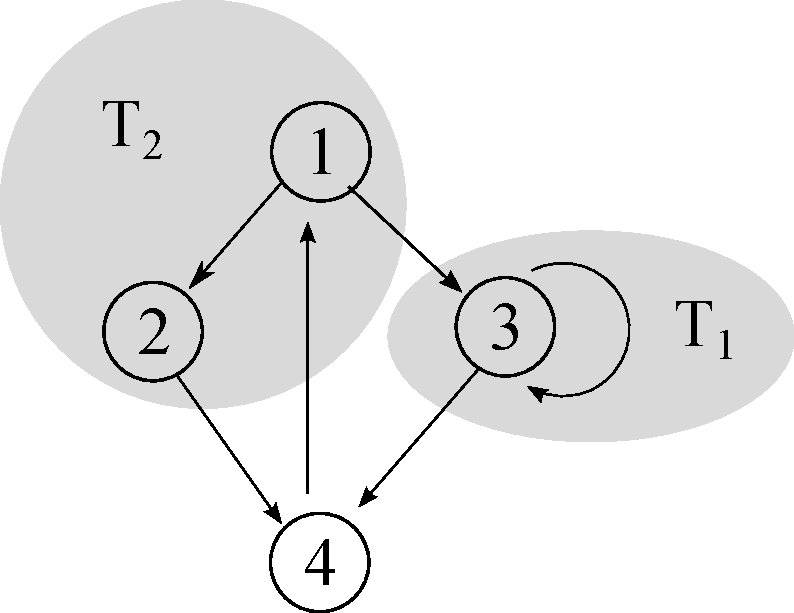
\includegraphics[width=5cm]{img/t1t2-1.pdf}
\end{center}
\caption{T$_{1}$-T$_{2}$-reduction}
\label{fig:t1t2-1}
\end{figure}

\subsection{Dataflow rules}

We will track the following pieces of information.\fxnote{All of this
  can be done in one pass - explain how and why.}

\begin{description}
\item[$\soacs : Exp \rightarrow (Label \times Pat \times Exp) Set$.]
  The set of all SOAC expressions that appears in an expression,
  modelled as a mapping from a (unique) label to a pair of a SOAC
  expression and its output pattern.  We shall say $\soacs(e)$ to
  refer to this mapping, and $\soacs(e)[l]$ to refer to the SOAC with
  label $l$.  For example,
  \begin{align*}
  & \soacs(\texttt{let \{$a$,$b$,$c$\} = mapT($f$,$x$,$y$,$z$) in \{$a$,$b$,$c$\}}) =\\
  & \quad \{ (\ell, \texttt{\{$a$,$b$,$c$\}},\texttt{mapT($f$,$x$,$y$,$z$)}) \},
  \end{align*}
  where $\ell$ is a fresh label.  After the $\soacs$ set has been
  computed, we can use $\soacs(e_{b})$, where $e_{b}$ is the body of a
  function to refer to the set of all SOACS in that function.  Since
  the fusion transformation is strictly intraprocedural, this is
  sufficient for our needs.

\item[$\infusible : Exp \rightarrow Name Set$.] The \textit{infusible
    set}, a set of variable names, is key to preventing unwanted
  fusion, as it indicates which SOACs should never be fused.  The
  infusible set prevents both undesired and invalid fusion, as
  outlined in sections \cref{sec:whentofuse,sec:invalidfusion}
  respectively.  Given an \LO{} expression $e$, we shall say
  $\infusible(e)$ to refer to the infusible set produced by $e$.  For
  example:
  \begin{align*}
  \infusible(&\texttt{let x = mapT(f,a) in}\\
  &\texttt{let y = mapT(g,a) in \{x,y\}}) = \{a\},
  \end{align*}
  because $a$ is used twice, and hence fusing its producer into
  \texttt{f} and \texttt{g} would cause work duplication.  To simplify
  the example, $f$ and $g$ are ignored when computing the infusible
  set, although as we shall see below, this is not the case in
  practice.

\item[$\inputs : Exp \rightarrow Name \rightarrow Labels$.] A mapping from arrays to a set of the SOACs that use the array
  as input.  This is modelled as a set of pairs, each pair consisting
  of an array name and a SOAC name.  We shall refer to the mapping
  generated by a given expression $e$ as $\inputs(e)$.  For example,
  \[
  \inputs(\texttt{mapT($f$, $x$, $y$, $z$)}) = \{ (x, \{\ell\}), (y, \{\ell\}), (z, \{\ell\}) \},
  \]
  where $\ell$ is the label of the \texttt{mapT}-SOAC.

  We define an associative and commutative operation $\sqcup$ to
  combine input mappings by taking the union of values (sets of
  labels, $s$) of corresponding keys (variable names, $v$), as
  follows.
  \begin{align*}
  &\{(v_{1},s_{1}),\ldots,(v_{n},s_{n})\} \sqcup \{(v_{n+1},s_{n+1}),\ldots,(v_{n+m},s_{n+m})\} =\\
  &\quad \{(v_{i}, \bigcup_{(v_{i},s_{j}),0 \leq j \leq n+m} s_{j})\},
  \end{align*}

  Intuitively, $x \sqcup y$ is a mapping that contains the union of
  the keys in $x$ and $y$, with the value for a key $v$ being the
  union of the values for $v$ in $x$ and $y$ (or just an untouched
  value, if $v$ was only present in one of the mappings).

  Similarly, we use $\sqcap$ to denote a similar mapping, except
  taking the intersection of values.
\begin{align*}
  &\{(v_{1},s_{1}),\ldots,(v_{n},s_{n})\} \sqcap \{(v_{n+1},s_{n+1}),\ldots,(v_{n+m},s_{n+m})\} =\\
  &\quad \{(v_{i}, \bigcap_{(v_{i},s_{j}),0 \leq j \leq n+m} s_{j})\},
  \end{align*}
\end{description}

If more specific rules are not given, the data flows default to the
following.

\begin{align*}
  \infusible(e) &= \bigcup_{e'\in\childExps{e}} \infusible(e') \\
  \\
  \inputs(e) &= \bigsqcup_{e'\in\childExps{e}} e'\\
  \\
  \soacs(e) &= \bigcup_{e'\in\childExps{e}} \soacs(e')
\end{align*}
Where $\childExps{e}$ are the \textit{immediate} children of $e$, e.g.
\[
\childExps{\texttt{if p(x) then t(y) else f(z)}} = \{\texttt{p(x)}, \texttt{t(y)}, \texttt{f(z)}\}.
\]

Now for specific rules, based on the shape of the given expression.

\begin{description}[style=nextline]
\item[Case $e \equiv v$ ($v$ is a variable)]

  This rule is only applied when $v$ is not an array input to a SOAC.
  This implies that the producer of $v$ cannot be fused, as its output
  $v$ is used here.
\begin{align*}
  & \infusible(e) = \{v\} \\
\end{align*}

\item[Case $e \equiv \texttt{$v$[$e_{1}$, \ldots, $e_{n}$]}$]

  If an element is retrieved from an array through indexing, we have
  no choice but to manifest that array, thus forcing us to avoid
  fusion due to our principle of avoiding duplication of computation.
  In many cases, for example if the array $v$ is the result of a
  \texttt{map} operation, it might be beneficial to replace the index
  operation by an inlined copy of the \texttt{map} function, and let
  the original \texttt{map} be fused.  Duplicating computation of a
  single element is likely acceptable, but not done in the general
  case by the current implementation, and it is hard to determine the
  optimal choice as long as \LO{} does not yet have a well-defined
  cost model.  Nevertheless, \cref{sec:inlining-indexing} will
  describe how we inline particularly simple cases.
  \begin{align*}
  & \infusible(e) = \{v\} \cup \bigcup_{1\leq i \leq n}\infusible(e_{i}) \\
\end{align*}

\item[Case $e \equiv \texttt{if $e_{c}$ then $e_{t}$ else $e_{f}$}$]

  The \infusible{} of a conditional consists of whatever is in the
  \infusible{} sets of its branches, plus any SOAC outputs that may be
  used multiple times.  Note that an output can be used in both the
  true and the false branch, and it will still only have been
  considered to be used once, becase only one of the true and false
  branch will be executed, never both.

\fixme{ArrInputs stuff not clear.}

\begin{align*}
  & \inputs(e) =\\
  & \quad \{ (v,s')\ |\ (v,s) \in \inputs(e_{t}) \cup \inputs(e_{f}) \}\\
  & \quad\quad \text{Where $s'$ is the set of all SOAC consumers of $v$ in both $e_{t}$ and $e_{f}$.} \\
  \\
  & \infusible(e) =\\
  & \quad \infusible(e_{c}) \cup \infusible(e_{t}) \cup \infusible(e_{f})\\
  & \quad \cup (\inputs(e_{c}) \sqcap \inputs(e_{t}))\\
  & \quad \cup (\inputs(e_{c}) \sqcap \inputs(e_{f}))\\
\end{align*}

The reason for these rules can be illustrated by the following
examples.  In \cref{fig:fuse-across-if-ok}, it is clear that fusing
computation of \texttt{b} with both \texttt{map(g,b)} and
\texttt{map(h,b)} will not cause duplicated computation, as the two
consumers are on separate control-flow paths.  On the other hand, if
even one branch contains multiple uses, as in
\cref{fig:fuse-across-if-bad}, we should not fuse.  Additionally, if
both the conditional expression and a branch consumes the same array,
as on \cref{fig:fuse-across-if-bad-condition}, then we should also not
fuse.

\begin{figure}
\begin{center}
\begin{bcolorcode}
let b = map(f, a) in
if p(x) then map(g,b)
        else map(h,b)
\end{bcolorcode}
\end{center}
\caption{Fusion into branches acceptable}
\label{fig:fuse-across-if-ok}
\end{figure}

\begin{figure}
\begin{center}
\begin{bcolorcode}
let b = map(f, a) in
if p(x) then concat(map(g,b),map(v,b))
        else map(h,b)
\end{bcolorcode}
\end{center}
\caption{Duplicating computation in one branch}
\label{fig:fuse-across-if-bad}
\end{figure}

\begin{figure}
\begin{center}
\begin{bcolorcode}
let b = map(f, a) in
if p(map(v,b)) then map(g,b)
               else map(h,b)
\end{bcolorcode}
\end{center}
\caption{Duplicating computation in conditional}
\label{fig:fuse-across-if-bad-condition}
\end{figure}

\item[Case $e \equiv \texttt{loop ($p$ = $e_{1}$) = for $v$ < $e_{2}$ do $e_{3}$ in $e_{4}$}$]

  For loops, we add any arrays used as SOAC inputs in the loop body to
  the infusible set.  This is because fusing into the loop would
  duplicate computation by re-evaluating the function in the consumer
  for every iteration of the loop -- see \cref{fig:cannot-fuse-loop}
  for an example of this.  This is similar to how we ban fusing into
  SOAC-functions.

  Note that any use of an array for another purpose than as SOAC input
  results in that array name being present in $\infusible(e_{3})$
  already, thus banning fusion.
\begin{align*}
  & \infusible(e) =\\
  & \quad \infusible(e_{1}) \cup \infusible(e_{2}) \cup \infusible(e_{3}) \cup \infusible(e_{4}) \\
  & \quad \cup \{ v\ |\ (v,s) \in \inputs(e_{3}) \}
\end{align*}

\begin{figure}
\begin{center}
\begin{bcolorcode}
let b = \emphh{map(f, a)} in
loop (v) = for i < n do
             let c = \emp{map(g, b)} in
             h(v,c) in
...
\end{bcolorcode}
\end{center}
\caption{Fusing the \emphh{producer} into the \emp{consumer} in the loop body would duplicate computation}
\label{fig:cannot-fuse-loop}
\end{figure}

\item[Case $e \equiv \texttt{let \{$\overline{vs}$\} = $soac$ in $e_{b}$}$]

  The big question here is whether $soac$ can be fused as producer
  with something in $\soacs(e_{b})$.  In the following, $\ell_{p}$ is
  a fresh name.  Let
  \[
  \zeta = \bigcup_{v \in vs} \inputs(e_{b},v)
  \]
  be the set of the labels of all SOACs that contain at least one of
  our outputs in their input set.  Additionally, let $e_{f}$ be the
  body of the function of $soac$.  In case $soac$ is
  \texttt{redomapT}, the second function (the inner fold) is used, as
  this is the one that is actually composed.

  For all $\ell^{c}_{i} \in \zeta$, we find the corresponding triple
  $(\ell^{c}_{i},vs^{c}_{i},soac^{c}_{i})$ in $\soacs(e_{b})$.  We can check
  whether fusion is possible by determining whether the following
  judgement is derivable.

\[
   \fusesto
    {vs}
    {soac}
    {soac^{c}_{i}}
    {soac^{r}_{i}}
\]

In total, the following four conditions must all be upheld before we
can fuse:

\begin{enumerate}
\item There must be at least one consumer $soac^{c}_{i}$ with which we can fuse.
\item For each consumer $soac^{c}_{i}$, we must be able to fuse and
  and get some $soac^{r}_{i}$.
\item None of $\overline{vs}$ are in the infusible set.  That is, if the intersection
\[
\overline{vs} \cap \infusible(e_{b})
\]
must be non-empty
\item No $soac^{r}_{i}$ uses an array past a point of consumption. \fixme{Um, detail how we track this.}
\end{enumerate}

\begin{description}
\item[If the four conditions are true:]

  In this case, we are fusing with several SOACs $soac_{c}$, each with
  a corresponding label $\ell_{c}$, and fused as $soac_{c_{r}}$.

\begin{align*}
  & \soacs(e) =\\
  & \quad (\soacs(e_{b}) \backslash \zeta)\\
  & \quad \cup \soacs(e_{f})\\
  & \quad \cup \{ (\ell_{c}, (vs, soac_{r}))\ |\ \textrm{for each $soac_{c_{r}}$} \}\\
  \\
  & \inputs(e) =\\
  & \quad (\textrm{$\inputs(e_{b})$ with all mappings to each $\ell_{c}$ removed}) \\
  & \quad \sqcup \{ (v,\ell_{c})\ |\ \textrm{for all array inputs $v$ in each $soac_{c_{r}}$} \}\\
  \\
  & \infusible(e) =\\
  & \quad \infusible(e_{b})\\
  & \quad \cup \{ v\ |\ (v,s) \in \inputs(e_{f}) \} \\
\end{align*}

\item[If they are not:]

  We cannot fuse with $soac$ as a producer, and we must add it as a
  kernel by itself.  It may be fused as the consumer at some later
  stage of the algorithm, however.

\begin{align*}
  & \infusible(e) =\\
  & \quad \infusible(e_{b})\\
  & \quad \cup \{ v\ |\ (v,s) \in \inputs(e_{f}) \} \\
  & \quad \cup \{ v\ |\ \textrm{$v$ is used as input to $soac$ but is also in $\inputs(e_{b})$} \}\\
  \\
  & \inputs(e) =\\
  & \quad \inputs(e_{b})\\
  & \quad \sqcup \inputs(e_{f})\\
  & \quad \sqcup \{(e_{1},\{\ell_{p}\}), \ldots, (e_{n},\{\ell_{p}\})\}\\
  \\
  & \soacs(e) = \soacs(e_{b}) \cup \{(\ell_{p}, (vs, soac))\} \\
  &
\end{align*}
\end{description}\fixme{infusible rule is still too unclear.}

\item[Case $e \equiv \texttt{let $v_{1}$ = $v_{2}$ with [$e_{1}$,\ldots,$e_{n}$] <- $e_{v}$ in $e_b$}$]

Record the in-place modification of $v_{2}$. \fxnote{Not sure how to model this yet.}

\end{description}

%%% Local Variables: 
%%% mode: latex
%%% TeX-master: "thesis.tex"
%%% End: 
